
\section{Formal system model in BIP}

In this section, we introduce an airplane engine control software case study. 
 For presentation simplicity, we choose one of its subsystems, the PLA signal processing system, as representative. 
 We will give an informal description, focusing on its functional structure, properties and conditional constraints. 
 Then we give the formal design model in BIP. 
 Finally, we provide model verfication and validation.


\subsection{Overview of the system model}

We construct the BIP model of the PLA signal processing system through the composition of atomic and composite components with BIP connectors. 
 The block diagram for our system is shown in Fig.1, it consists of a Task Unit and a Signal Processing Unit. 
 The Signal Processing Unit consists of atomic component c1, composite components p1 and c2. 
 In the Task Unit, there is an atomic component t1, which produce signal value for Signal Processing Unit.

\begin{figure}[ht!]
	\centering
	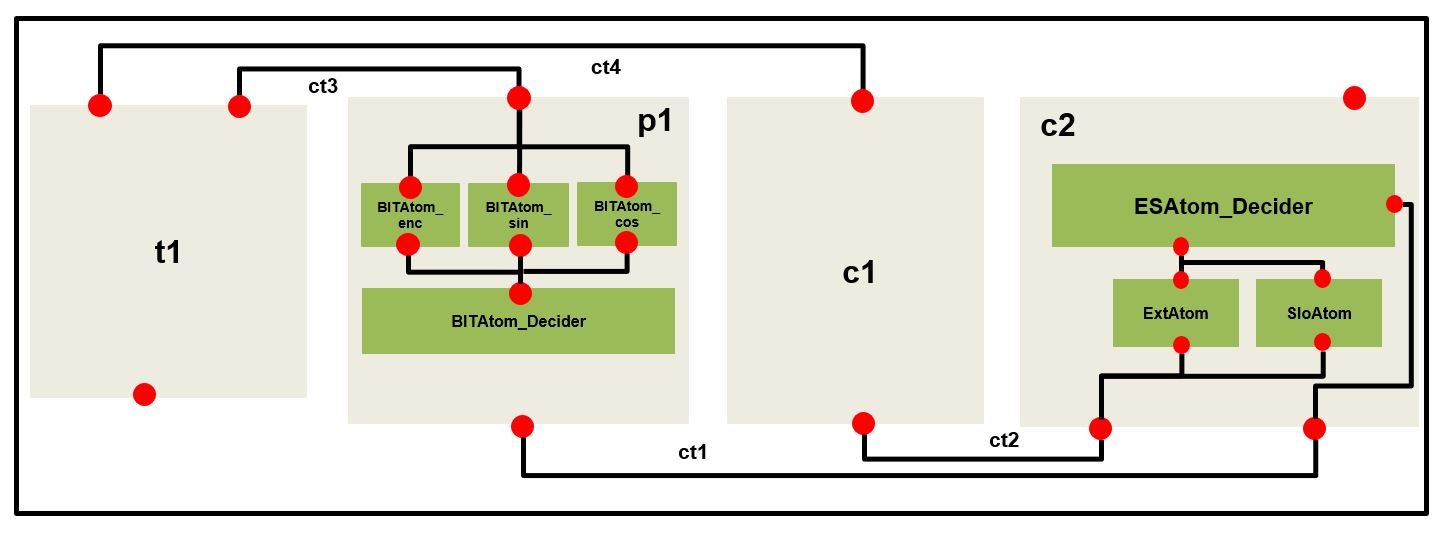
\includegraphics[width=90mm]{figure/figure2.jpg}
	\caption{System Architecture}
	\label{Sys_Model}
\end{figure}

\begin{comment}
The atomic components of our system are \emph{TaskAtom t1}, \emph{CalibrationAtom c1} and several atomics in \emph{p1} and \emph{c2}. For each atomic component, we specify its ports, variables and behavior.
\end{comment}

\begin{figure}[ht!]
	\centering
	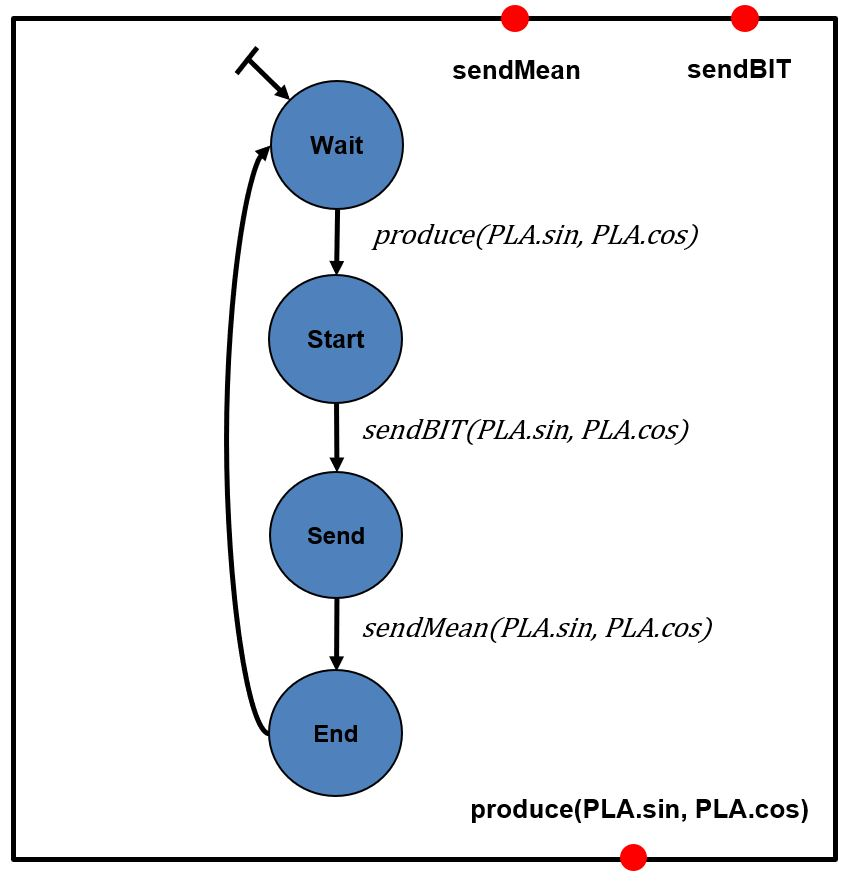
\includegraphics[width=50mm]{figure/figure3.jpg}
	\caption{The Task Component}
	\label{Task_Component}
\end{figure}

The behavior of atomic component t1 is shown in Fig.2. It is used as simulator of the input stimuli. In the graphical notation, the atomic is initialized to \emph{Wait}, and the following three transitions are driven by corrensponding events: \emph{produce}, \emph{sendBIT} and \emph{sendMean}, which represents three corrensponding ports in the atomic. For instance, whenever the current state is at \emph{Start}, the port \emph{sendBIT} will be activated and the transition will be executed once the event \emph{sendBIT} is done.

\begin{figure}[ht!]
	\centering
	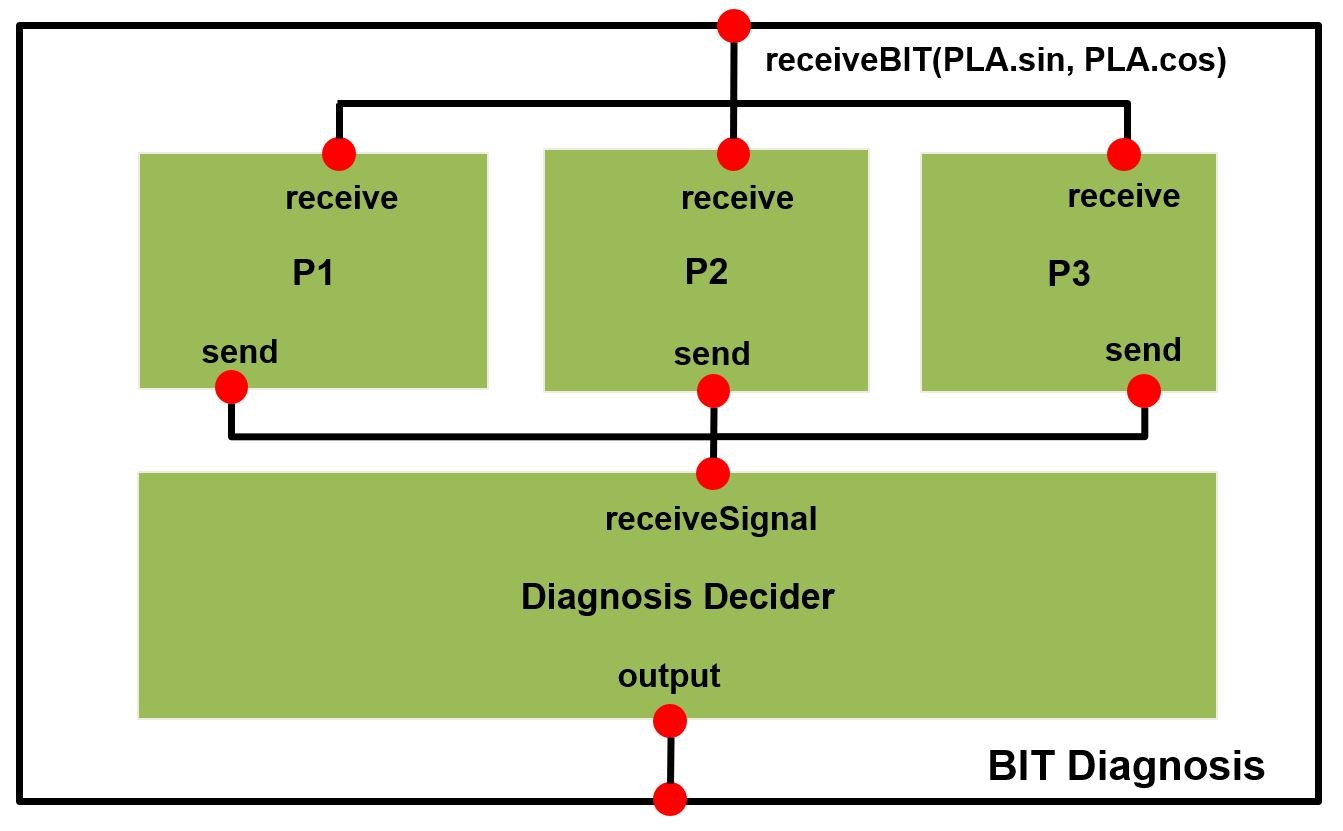
\includegraphics[width=80mm]{figure/figure4.jpg}
	\caption{Architecture of BIT Diagnosis}
	\label{BIT_Model}
\end{figure}

\subsubsection{BIT Diagnosis module}


\noindent In our design, the BIT Diagnosis module, Calibration Conversion module and Extremum/Slope Diagnosis module are three subsystems of PLA signal processing system. The BIT Diagnosis module is shown in figure 3. In the graphical notation, the three atomic component instances \emph{p1}, \emph{p2} and \emph{p3} receive BIT signal through port \emph{receiveBIT}, a connector distributes the signal to these components and another connector merges their output and sends it to the an instance of \emph{Decider} component. The BIP description of the definition and instantiation of \emph{BIT Diagnosis} is shown below:

\begin{lstlisting}
`\textbf{compound} \emph{BITCompound\_P1}`
  `\textbf{component} \emph{BITAtom\_enc enc}`
  `\textbf{component} \emph{BITAtom\_sin sin}`
  `\textbf{component} \emph{BITAtom\_cos cos}`
  `\textbf{component} \emph{BITAtom\_Decider d}`

  `\textbf{connector} \emph{ThreeToOne o(enc.sendBIT,sin.sendBIT,cos.sendBIT,d.receiveSignal)}`
  `\textbf{connector} \emph{Merge m(enc.receiveBIT,sin.receiveBIT,cos.receiveBIT)}`

  `\textbf{export port} \emph{m.Merged\_Signal} \textbf{as} \emph{receiveBIT}`
  `\textbf{export port} \emph{d.output} \textbf{as} \emph{sendBIT}`
`\textbf{end}`
\end{lstlisting}

We define the two ports in \emph{BITCompound\_P1} as export to give them an external property which enables them to be triggered by other components.

\begin{lstlisting}
`\textbf{connector type} \emph{ThreeToOne(PLAPort\_t1 r1, PLAPort\_t1 r2, PLAPort\_t1 r3, PLAPort\_t3 r4)}`
  `\textbf{define} \emph{r1 r2 r3 r4}`
  `\textbf{on} \emph{r1 r2 r3 r4} \textbf{down} \emph{\{r4.a=r1.a; r4.b=r2.a; r4.c=r3.a;\}}`
`\textbf{end}`
\end{lstlisting}

\begin{lstlisting}
`\textbf{connector type} \emph{Merge(PLAPort\_t2 r1, PLAPort\_t2 r2, PLAPort\_t2 r3)}`
  `\textbf{data int} \emph{mysin,mycos}`
  `\textbf{export port} \emph{PLAPort\_t2 Merged\_Signal(mysin,mycos)}`
  `\textbf{define} \emph{r1 r2 r3}`
  `\textbf{on} \emph{r1 r2 r3} \textbf{down} \emph{\{r1.a=mysin; r2.a=mysin; r3.a=mysin; r1.b=mycos; r2.b=mycos; r3.b=mycos;\}}`
`\textbf{end}`
\end{lstlisting}

In our system, atomic component is considered as the smallest unit of the architecture, while in the combination of several components, such as our BIT Diagnosis module, we have to ensure that the output of three components can simultaneously reach the connoector, otherwise it will fall into deadlock status. To avoid this problem, the three atomic components are designed homogeneous, we take one of these three components, \emph{BITAtom\_enc p1}, as an example, its ports and behavior is shown below:

\begin{figure}[ht!]
	\centering
	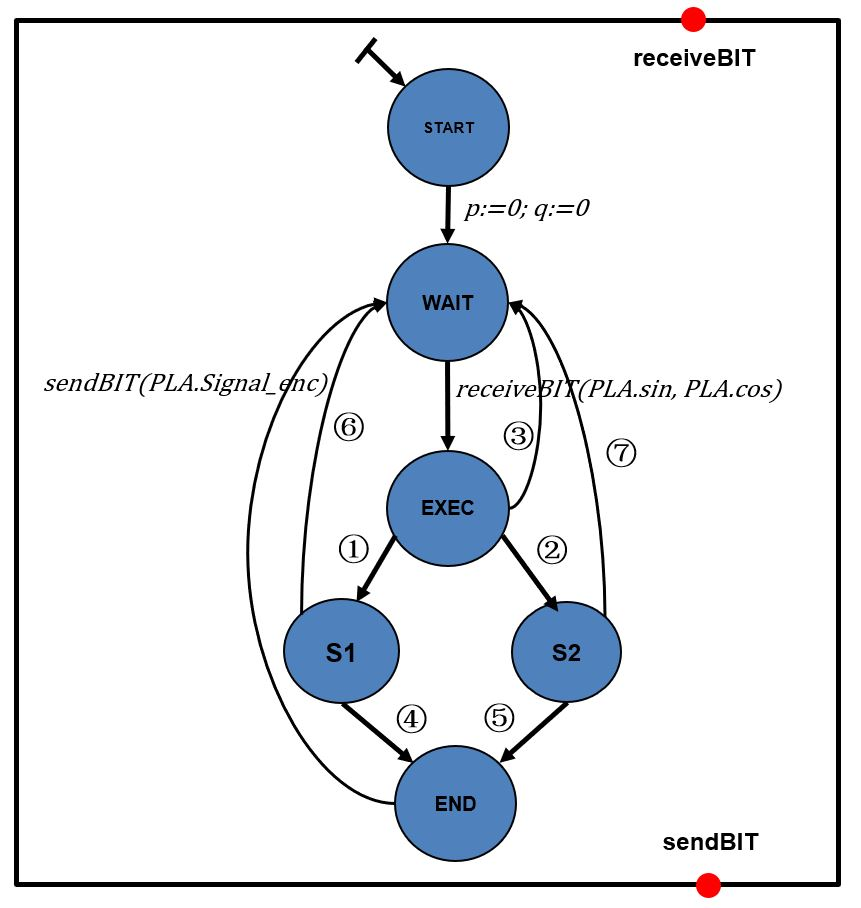
\includegraphics[width=60mm]{figure/figure5.jpg}
	\caption{BIT Diagnosis P1}
	\label{BIT_enc_Model}
\end{figure}
\begin{table}[]
	\vspace{20pt}
	\caption{Transitions of P1}
	\centering
	\begin{tabular}{lllll}
		\hline
		\thead[l]{Transition} & \thead[l]{Guard}& \thead[l]{Action}
		\\
		\hline
		1  & PLA.sin $<500 \wedge$ PLA.cos $<500$   & $p :=p+1 ; q :=0$ \\
		2  & PLA.sin $>=500 \wedge$ PLA.cos $>=500$   & $p :=0 ; q :=q+1$ \\
		3  & PLA.sin $ >=500 \oplus$ PLA.cos $>=500$   & $p :=0 ; q :=0$ \\
		4  & $p>=5$   & PLA.Signal\_enc: $=1$ \\
		5  & $q>=5$   & PLA.Signal\_enc: $=0$ \\
		6  & $p<5$   & null \\
		7  & $q<5$   & null \\
		\hline
	\end{tabular}
	\label{bs}
\end{table}

During execution, we consider a WAIT to WAIT transition set as a cycle. In each cycle, we ensure that an \emph{sendBIT} event will be activated to avoid the system falling into deadlock status. With the combination of connector, \emph{P1} gives a synchronous output together with other two atomic component instances. We define two variables \emph{p} and \emph{q} as counters to control the vary of signal. Their constraint indicates that for every continuous five cycles, the system does a setting and gives a corresponding output through port \emph{sendBIT}.

\begin{figure}[ht!]
	\centering
	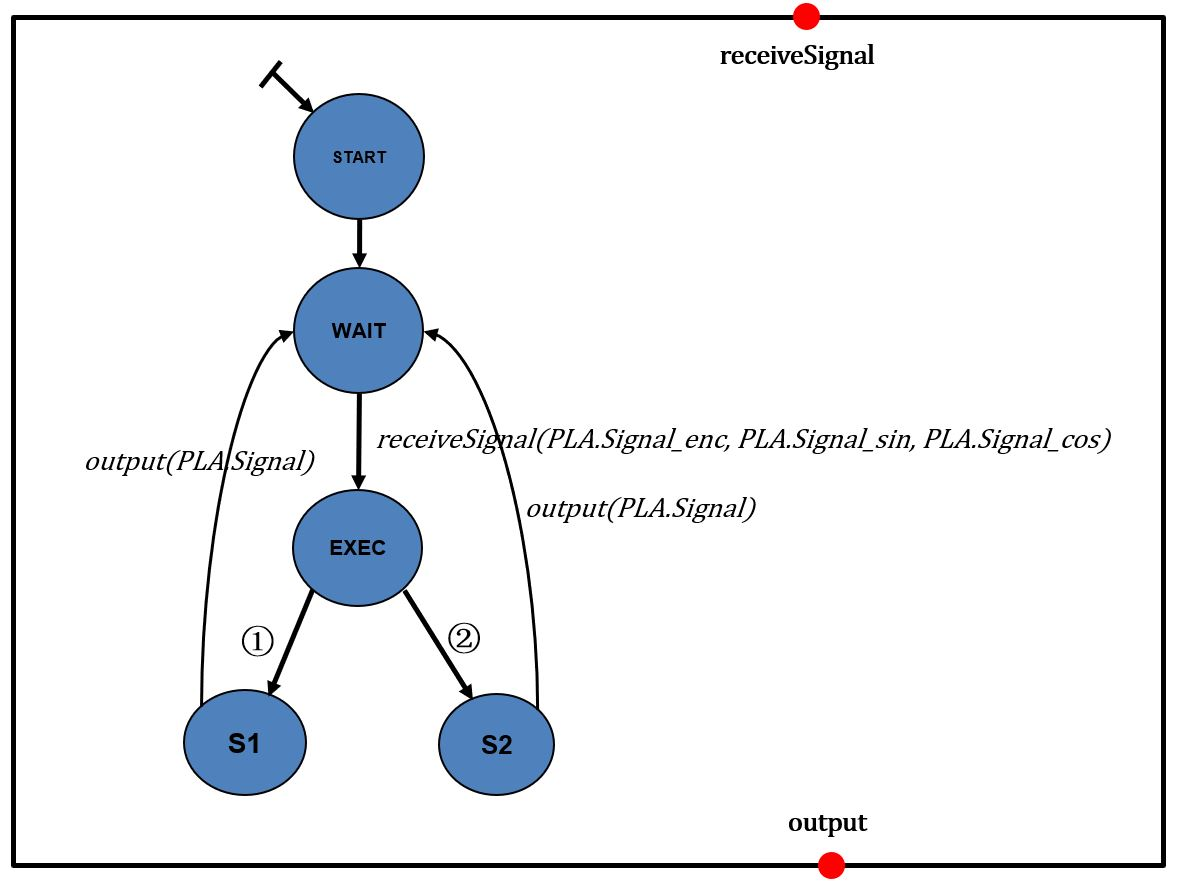
\includegraphics[width=60mm]{figure/figure6.jpg}
	\caption{BIT Diagnosis Decider}
	\label{BIT_decider_Model}
\end{figure}

\begin{table}[]
	\vspace{20pt}
	\caption{Transitions of Decider}
	\centering
	\begin{tabular}{lllll}
		\hline
		\thead[l]{Transition} & \thead[l]{Guard}& \thead[l]{Action}
		\\
		\hline
		1  & PLA.Signal\_enc $=0 \wedge$ PLA.Signal\_sin $=0 \wedge$ PLA.Signal\_cos $=0$  & $PLA.Signal :=0$ \\
		2  & PLA.Signal\_enc $=1 \vee$ PLA.Signal\_sin $=1 \vee$ PLA.Signal\_cos $=1$   & $PLA.Signal :=1$ \\
		\hline
	\end{tabular}
	\label{bs}
\end{table}

As shown in Fig.5, the BIT Diagnosis Decider is responsible for integrating the signals output by three BIT Diagnosis. We also produce a WAIT to WAIT transition set, \emph{receiveSignal} as input event and \emph{output} as output event. We define a bool type variable \emph{PLA.Signal} as the BIT fault signal for output.

\subsubsection{Calibration Conversion module}

\

\

\noindent The Calibration Conversion module collects the signal from signal collector and converts it to the corresponding engineering value by means of a calibration curve and an index table. This module is designed as an atomic component c1 in the BIP model, its ports and behavior is shown below:

\begin{figure}[ht!]
	\centering
	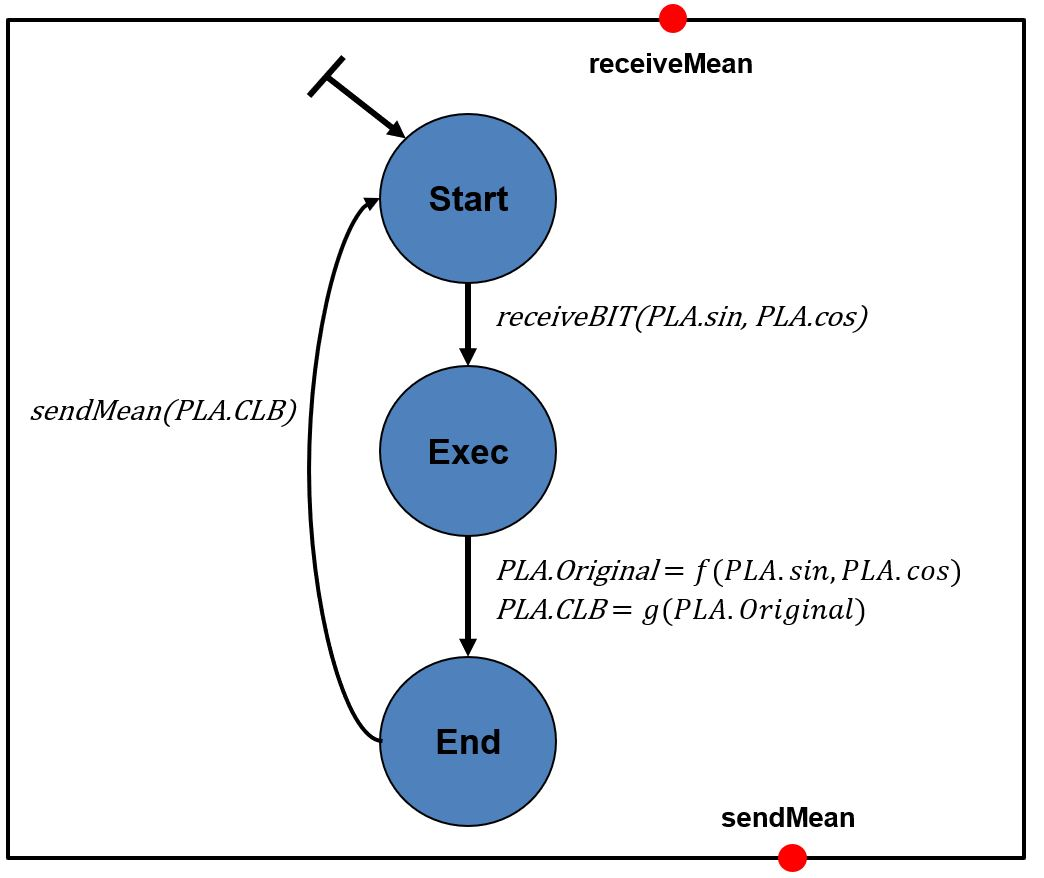
\includegraphics[width=60mm]{figure/figure7.jpg}
	\caption{Calibration conversion module}
	\label{Calibration_conversion}
\end{figure}

It has been introduced that every atomic component can be converted to its corresponding BIP description. The BIP description of the definition of \emph{Calibration Conversion} is shown below:

\begin{lstlisting}
`\textbf{atom} \emph{CalAtom}`
  `\textbf{data int} \emph{mysin,mycos}`
  `\textbf{data int} \emph{myangle}`

  `\textbf{export port} \emph{PLAPort\_t2 receiveMean(mysin,mycos)}`
  `\textbf{export port} \emph{PLAPort\_t4 sendMean(myangle)}`

  `\textbf{place} \emph{START, EXEC, END}`

  `\textbf{initial to} \emph{START}`
    `\textbf{do} \emph{\{myangle = 0;\}}`

  `\textbf{on} \emph{receiveMean} \textbf{from} \emph{START} \textbf{to} \emph{EXEC}`

  `\textbf{internal from} \emph{START} \textbf{to} \emph{EXEC}`
    `\textbf{do} \emph{\{myangle = mysin * mycos + 1;\}}`

  `\textbf{on} \emph{sendMean} \textbf{from} \emph{END} \textbf{to} \emph{START}`
`\textbf{end}`
\end{lstlisting}

In the BIP description, we define internal data, external ports, serveral states and transitions. Transitions begin with field \emph{on} are external transitions which are driven by external events. Relatively, transitions begin with field \emph{internal} literally internal transitions which are executed as soon as the atomic component reach the state. We define an internal variable \emph{myangle} for output. System calculate its value through calibration curve and index table from two variables \emph{mysin} and \emph{mycos}.

\subsubsection{Extremum/Slope Diagnosis module}

\

\

\noindent The Extremum/Slope Diagnosis module is almost the same as BIT Diagnosis module. It picks up signal value, diagnoses them and integrates the results into one variable for output. We also provide the architecture of Extremum/Slope Diagnosis:

\begin{figure}[ht!]
	\centering
	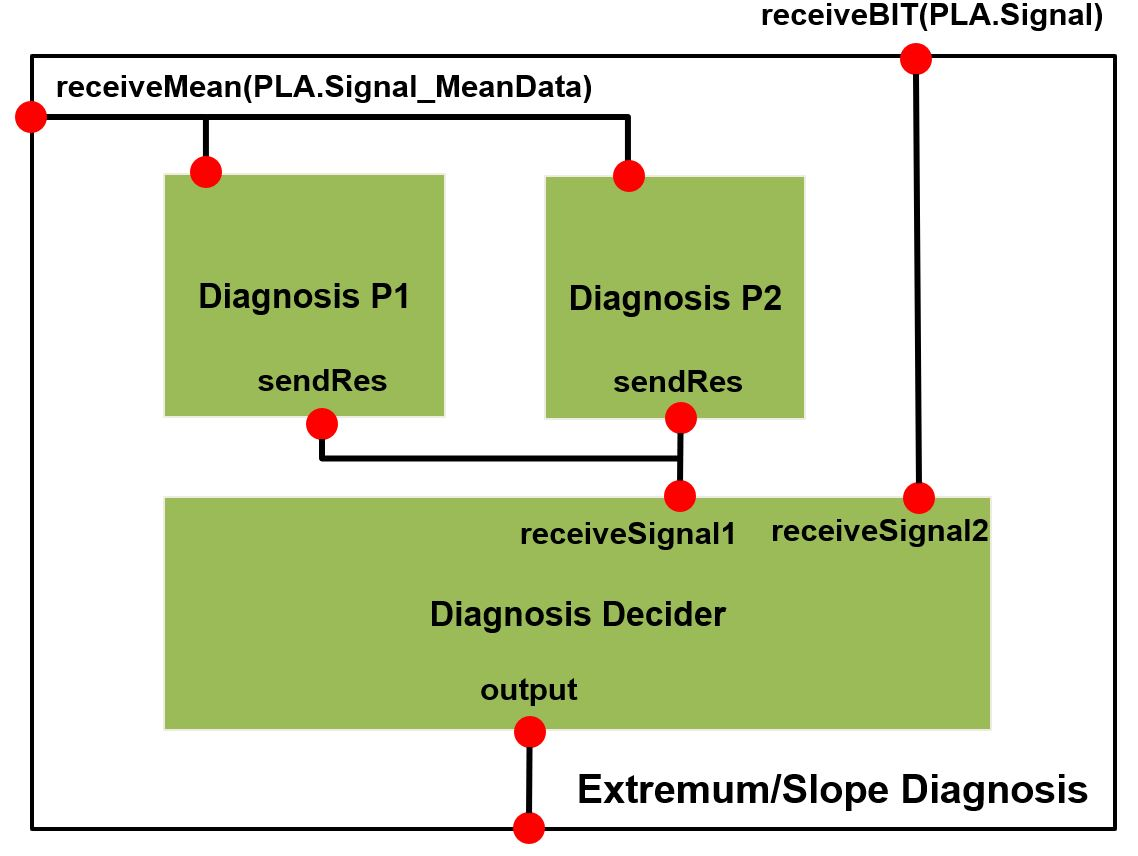
\includegraphics[width=90mm]{figure/figure8.jpg}
	\caption{Architecture of Extremum/Slope Diagnosis}
	\label{Ext/Slo_module}
\end{figure}

It should be noticed that in Extremum/Slope Diagnosis module, besides signals sent by internal atomic components p1 and p2, the \emph{Decider} also pick up signal from BIT Diagnosis module as input. We give the BIP Description of the Extremum/Slope Diagnosis module below:

\begin{lstlisting}
`\textbf{compound} \emph{ESCompound\_C1}`
  `\textbf{component} \emph{ExtAtom enc}`
  `\textbf{component} \emph{SloAtom slo}`
  `\textbf{component} \emph{ESAtom\_Decider d}`

  `\textbf{connector} \emph{TwoToOne o(ext.sendRes,slo.sendRes,d.receiveSignal1)}`
  `\textbf{connector} \emph{Merge\_two m(ext.receiveMean,slo.receiveMean)}`

  `\textbf{export port} \emph{d.receiveSignal2} \textbf{as} \emph{receiveBIT}`
  `\textbf{export port} \emph{m.Merged\_Signal\_two} \textbf{as} \emph{receiveMean}`
`\textbf{end}`
\end{lstlisting}

The connector types \emph{TwoToOne} and \emph{Merge\_two} do almost the same work as the two connector types used in BIT Diagnosis module except that the connector types used here have only two parameters, not three.

\
In the entire system, the compound type \emph{ESCompound} will be instantiated as c2, which is introduced in Fig.1.

\
Till now, we have introduced our system informally and in formal BIP description. To give a formal proof whether our system and BIP model is safety and effectiveness or not, the verification and validation of the system above will produced in the next chapter.
\subsection{Model verification and validation}

